\documentclass[10pt]{article}
\usepackage{fontspec}
\usepackage{polyglossia}
\setdefaultlanguage{french}
\usepackage[a4paper,margin=2cm]{geometry}
\usepackage{url,hyperref}
\usepackage{siunitx}
\usepackage{schemabloc}
\usepackage{listings}
\usepackage{auto-pst-pdf}
\usepackage{pst-circ}
\usepackage{soul}
\usepackage{verbatim}
\usepackage{lmodern}
\usepackage{tikz}
\usepackage[european,cuteinductors,siunitx]{circuitikz}
\usepackage{xunicode,xltxtra}
\usepackage{graphicx}
\usepackage{amsmath}
\usepackage{minted}
\usepackage{multicol}
\usepackage{float}
\floatplacement{figure}{H}
\title{
\includegraphics{../images/inp-enseeiht} \\ ~ \\ ~ \\ ~ \\ ~ \\
Pré-projet Professionnel}
\author{Guilhem Saurel}
\date{\today}
\renewcommand{\thesection}{\Roman{section}}
\renewcommand{\thesubsection}{\thesection .\alph{subsection}}
\begin{document}

\begin{titlepage}
    \maketitle
    \tableofcontents
\end{titlepage}

\section{}
\subsection{Je souhaite découvrir les 2 secteurs d’activité suivants}
Les deux secteurs d’activité qui m’intéressent le plus sont:
\begin{enumerate}
    \item Conception de processeurs (CPU/GPU/µC);
    \item Robotique (robots industriels de construction, domotique, aérospatiale,…)
\end{enumerate}
\subsection{J’ai envie d’exercer (ou de découvrir) les métiers suivants parmi ces 2 secteurs d’activité cités}
\begin{itemize}
    \item Ingénieur électronicien;
    \item Ingénieur en robotique;
    \item Ingénieur de recherche;
\end{itemize}

\section{Je présente le résultat de mes recherces bibliographiques au sujet de 2 de ces métiers}
\begin{figure}
    \begin{center}
        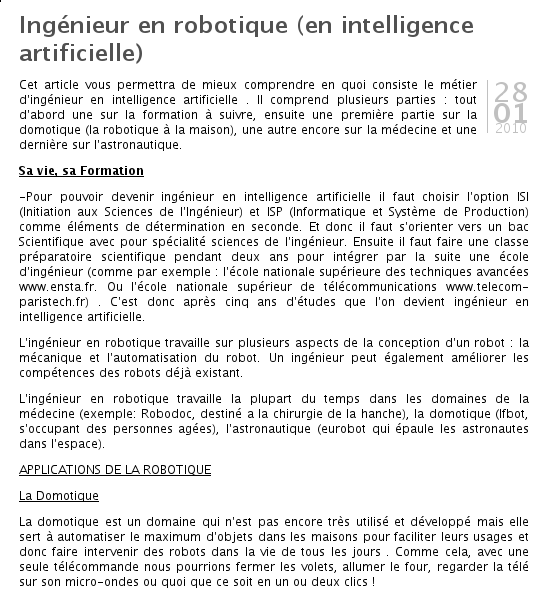
\includegraphics[width=10cm]{ir}
        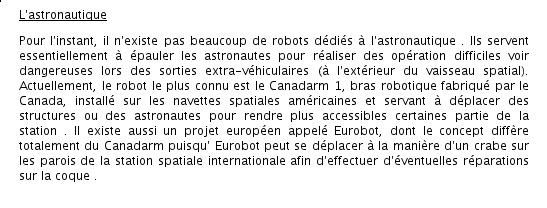
\includegraphics[width=10cm]{ir2}
    \end{center}
    \caption{Ingénieur en robotique}
    Source: http://blogs.onisep.fr/concours/concours\_blogs/prix/blogs\_2010/Lycee-Jean-Jaures789/index2e86.html?2010/01/28/8-ingenieur-en-robotique-en-intelligence-artificielle
\end{figure}
\begin{figure}
    \begin{center}
        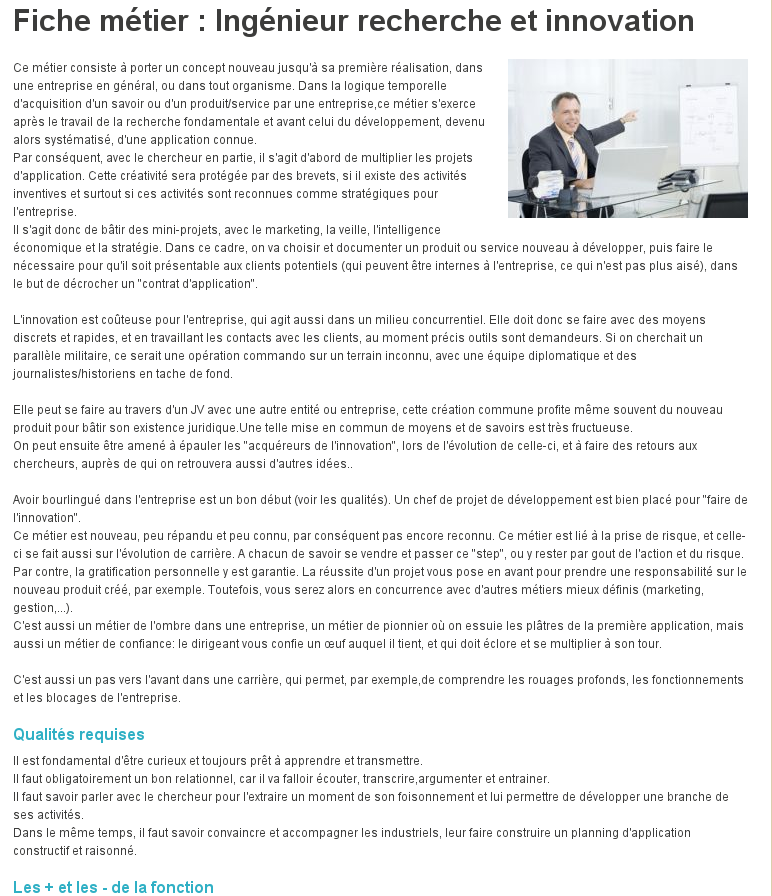
\includegraphics[width=10cm]{irech}
        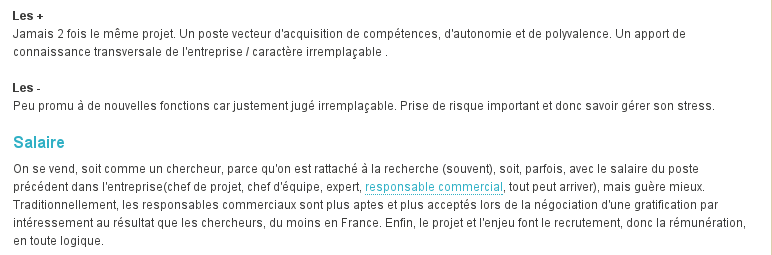
\includegraphics[width=10cm]{irech2}
    \end{center}
    \caption{Ingénieur de recherche}
    Source: http://www.blogdesmetiers.com/index.php/post/ingenieur-recherche-et-innovation
\end{figure}

\section{Je repère mes compétences}
À la fin de ma formation, j’aurai toutes les compétences d’un ingénieur INP-ENSEEIHT,
ainsi que celles spécifique à ma filière (électronique). J’aurai également beaucoup
appris aux clubs informatique et robotique, que ce soit sur au niveau des compétences
techniques ou sur le savoir être. J’ai également eu des postes à responsabilité dans ces
clubs (président, trésorier).

\section{Je précise les compléments de formation concernant: les poursuites d’études nécessaires,
les parcours pour faciliter mon intégration professionnelle dans les métiers étudiés ci-dessus}

Les différents parcours à envisager sont:
\begin{itemize}
    \item Thèse puis Labo;
    \item Thèse en CIFRE puis Labo ou grand groupe;
    \item PME puis grand groupe;
    \item Création d’entreprise;
\end{itemize}

\section{Je présente 2 offres d’emploi correspondant à chacun des 2 métiers explorés résultants d’une
    recherche internet ou presse spécialisée… Ainsi que 2 offres d’emploi correspondant à chacun des 2 métiers
explorés résultant de l’AIN7}

\begin{figure}
    \begin{center}
        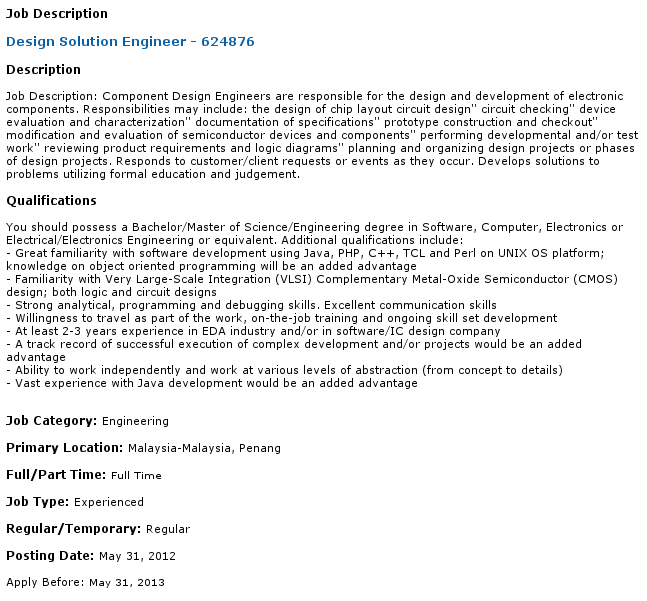
\includegraphics[width=10cm]{intel}
    \end{center}
    \caption{Design Solution Engineer}
    Source: http://www.intel.com/jobs/jobsearch/index.htm
\end{figure}

\begin{figure}
    \begin{center}
        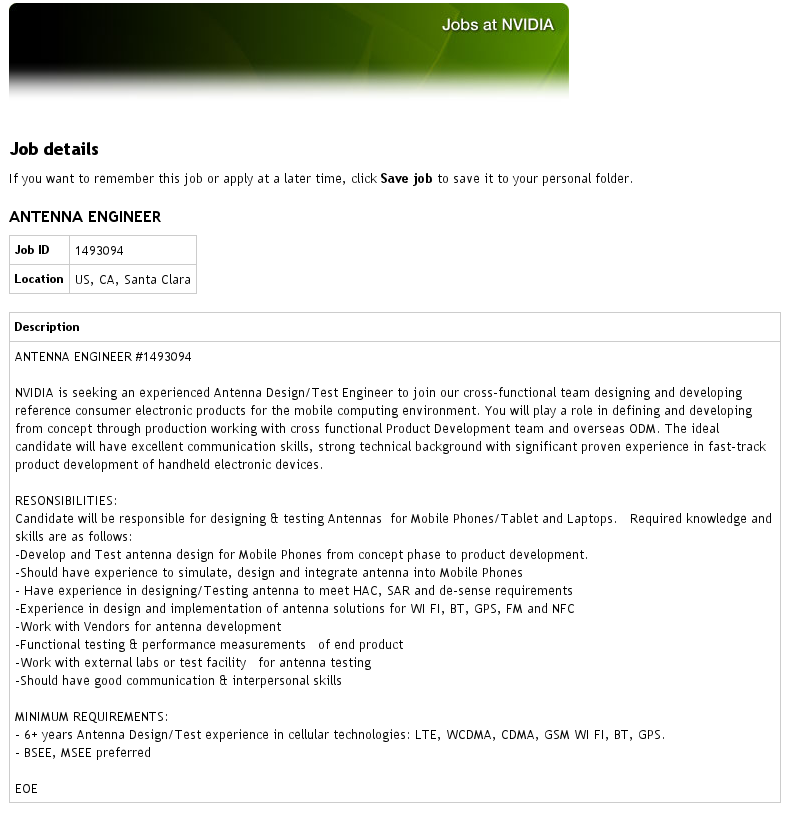
\includegraphics[width=10cm]{antenne}
    \end{center}
    \caption{Antenna Engineer}
    Source: http://careers.nvidia.com/pljb/global\_jsp/applicant/DisplayJob/JobDetails.jsp?display=1\&pljbHome=/nvidia/nvidiaemployment/applicant/index.jsp\&id=7382
\end{figure}

\section{Je note au moins 8 noms d’entreprises qu’il serait souhaitable de contacter pour effectuer un stage afin de
donner de la cohérence à un CV}
\begin{itemize}
    \item Nvidia;
    \item Intel;
    \item Samsung;
    \item HTC;
    \item CNES;
    \item CEA;
    \item Alsthom;
    \item Viveris;
\end{itemize}

\end{document}
